\documentclass{article}

\usepackage{color}
\usepackage{indentfirst}
\usepackage{graphicx}
\usepackage{amsmath}
\usepackage{geometry}
\usepackage{setspace}
\usepackage{indentfirst}
\usepackage{listings}
\usepackage{xcolor}
\lstset{
    columns=fixed,       
    numbers=left,                                       
    frame=none,                                          
    backgroundcolor=\color[RGB]{245,245,244},            
    keywordstyle=\color[RGB]{40,40,255},                 
    numberstyle=\footnotesize\color{darkgray},           
    commentstyle=\it\color[RGB]{0,96,96},                
    stringstyle=\rmfamily\slshape\color[RGB]{128,0,0},   
    showstringspaces=false,                              
    language=c++,                                        
}
\geometry{left=2cm,right=2cm,top=2cm,bottom=2cm}
\begin{document}
\begin{spacing}{2.0}
\vspace*{0.25cm}

\hrulefill

\thispagestyle{empty}

\begin{center}
\begin{large}
\sc{UM--SJTU Joint Institute \vspace{0.3em} \\ Data Structures and Algorithms \\(VE281)}
\end{large}

\hrulefill

\vspace*{5cm}
\begin{Large}
\sc{{Homework 3}}
\end{Large}

\vspace{2em}

\end{center}


\vfill

\begin{table}[h!]
\flushleft
\begin{tabular}{lll}
Name: Ji Xingyou \hspace*{2em}&
ID: 515370910197\hspace*{2em}
\\

Date: 6 November 2017

\end{tabular}
\end{table}

\hfill

\newpage
\tableofcontents
\newpage
\section{Theoretical Data}
\indent As is discussed in the class, we can get the following table summarizing the time complexity for each priority queues.
\subsection{binary\_heap}
\begin{table}[!hbp]
\centering
\begin{tabular}{c|c}
enqueue&$O(logN)$\\
\hline
dequeue\_min&$O(logN)$\\
\hline
get\_min&$O(1)$\\
\end{tabular}
\caption{Time complexity of binary\_heap.}
\end{table}
\subsection{unsorted\_heap}
\begin{table}[!hbp]
\centering
\begin{tabular}{c|c}
enqueue&$O(1)$\\
\hline
dequeue\_min&$O(N)$\\
\hline
get\_min&$O(N)$\\
\end{tabular}
\caption{Time complexity of unsorted\_heap.}
\end{table}
\subsection{fib\_heap}
\begin{table}[!hbp]
\centering
\begin{tabular}{c|c}
enqueue&$O(1)$\\
\hline
dequeue\_min&$O(logN)$\\
\hline
get\_min&$O(1)$\\
\end{tabular}
\caption{Time complexity of fib\_heap.}
\end{table}
In this report, we will first implement all these three priority queues, and then test the run time for each of them to see whether the above table makes sense.

The implementation of the priority queues is attached in the appendix.
\section{Result Analysis}
\indent After finishing implementing the above three priority queues, I wrote another program to test the run time of each priority queues. In this program, I set two clocks, noting the starting and finishing instance. To avoid uncertainty in the data, I wrote a while loop to run the program 10 times so that I could get the average value.

The grid size I chose is 16, 25, 100, 225, 400, 625, 900, 1600, 2500, 3600, 4900, 6400, 8100, 10000.

The run time data for each priority queues is listed in table 2.
\begin{table}[!h]
\centering
\begin{tabular}{c|ccc}
Grid size&binary\_heap&unsorted\_heap&fib\_heap\\
\hline
\hline
16&281&337&332\\
\hline
25&376&343&397\\
\hline
100&416&530&1386\\
\hline
225&493&691&2066\\
\hline
400&648&800&4493\\
\hline
625&793&926&8120\\
\hline
900&838&1175&11461\\
\hline
1600&867&1372&32847\\
\hline
2500&1417&2270&68225\\
\hline
3600&2180&3107&106249\\
\hline
4900&2329&4587&168253\\
\hline
6400&2364&5894&292624\\
\hline
8100&3397&8836&356320\\
\hline
10000&5692&9915&492132\\
\hline
22500&5849&26533&1891842\\
\hline
40000&9129&59409&3676906\\
\hline
\end{tabular}
\caption{Run time of priority queues}
\end{table}

The run time comparison is shown in figure 1. 

\begin{figure}[h!]
\begin{center}
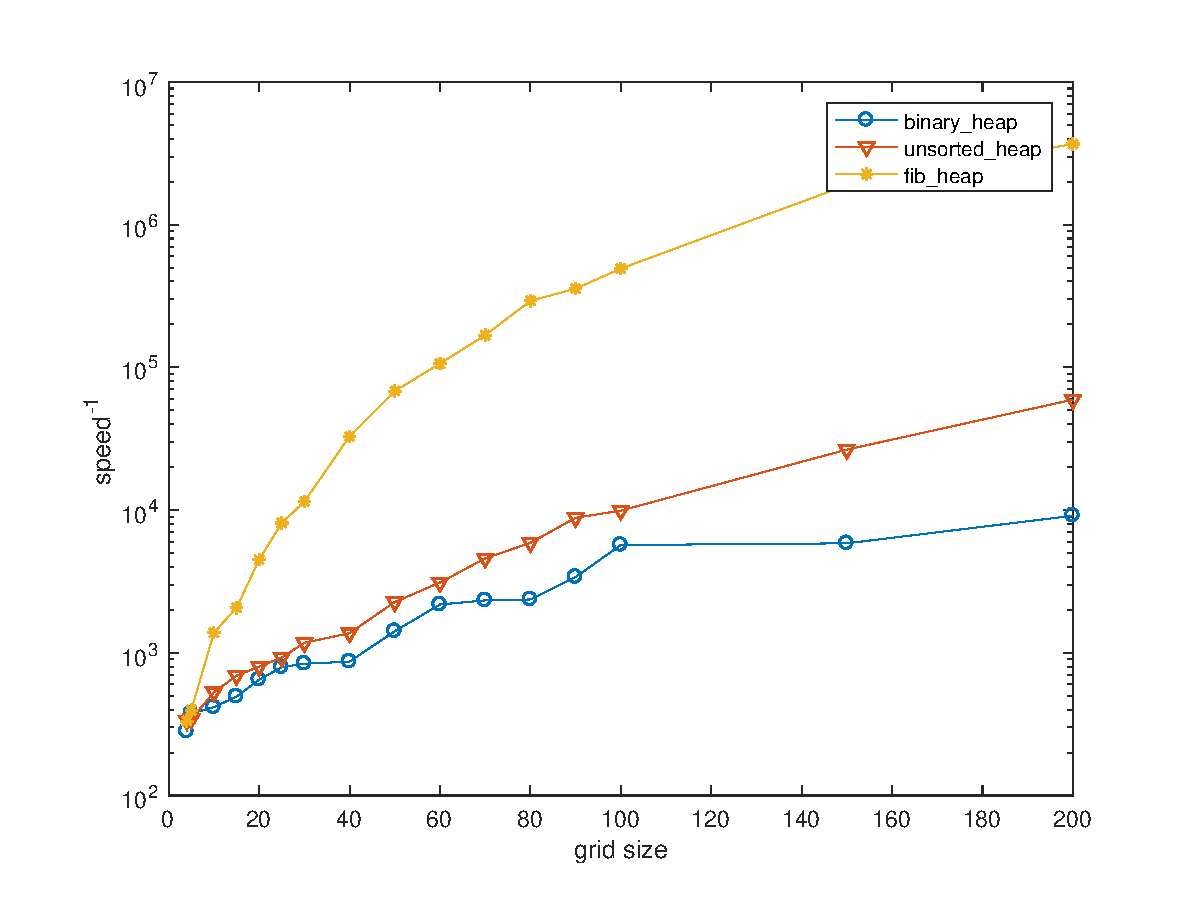
\includegraphics[scale=1]{PQ.eps}
\caption{Run time comparison}
\end{center}
\end{figure}

Combining the table and figure above, we can conclude the following points.
\begin{enumerate}
\item For each priority queue, the run time increases as the size of the grid increases.
\item For different grid size, binary\_heap has the best the performance among all while the fib\_heap has the worst.
\end{enumerate}

\indent However, for the reason that my fib\_heap is not well implemented, which I myself does not know where goes wrong, this does not cover the real situation.\\
\indent Below I will illustrate the real case, which can not be derived from my figure. The real cases are from the discussion with my classmates. All the conversation is conducted in a normal way which does not involve an Honor Code violation. Reference is available if requested.
\begin{enumerate}
\item When the grid size is small (less than 100), unsorted\_heap has a better performance than fib\_heap.
\item When the array size becomes gradually larger (greater than 100), fib\_heap has a better performance than unsorted\_heap.
\item No matter what the grid size is, binary\_heap always has the best performance among these three.
\end{enumerate}

This inspires me that in future learning, when dealing with priority queues, I should make a wise choice on which form to apply. For example, when the grid size is small, I should use binary\_heap or unsorted\_heap. When the grid size is large, I should choose Fibonacci\_heap or binary\_heap.
\section{Appendix}
\subsection{Priority queues}
\subsubsection{main.cpp}
\begin{lstlisting}[language=c++]
//
//  main.cpp
//  project3
//
//  Created by 季星佑 on 2017/10/27.
//  Copyright © 2017年 季星佑. All rights reserved.
//

#include <iostream>
#include <getopt.h>
#include "priority_queue.h"
#include "binary_heap.h"
#include "fib_heap.h"
#include "unsorted_heap.h"

using namespace std;

class point {
public:
    int x;
    int y;
    int cellweight=0;
    int pathcost=0;
    bool reached=false;
    point *predecessor=NULL;
    friend bool operator==(const point &p1,const point &p2)
    {
        return (p1.x==p2.x&&p1.y==p2.y&&p1.cellweight==p2.cellweight&&p1.pathcost==p2.pathcost&&p1.reached==p2.reached&&p1.predecessor==p2.predecessor);
    }
    friend bool operator<(const point &p1,const point &p2)
    {
        return p1.pathcost<p2.pathcost;
    }
    friend bool operator>(const point &p1,const point &p2)
    {
        return p1.pathcost>p2.pathcost;
    }
    struct compare_t
    {
        bool operator()(const point &a, const point &b) const
        {
            return (a.pathcost<b.pathcost)||((a.pathcost==b.pathcost)&&(a.x<b.x))||((a.pathcost==b.pathcost)&&(a.x==b.x)&&(a.y<b.y));
        }
    };
};

void trace_back_path(point *p);

int main(int argc,char* argv[])
{
    int width,height=0;
    cin>>width;
    cin>>height;
    int start_point_x,start_point_y,end_point_x,end_point_y;
    cin>>start_point_x>>start_point_y>>end_point_x>>end_point_y;
    point p_array[height][width];
    for(int h=0;h<height;++h)
    {
        for(int w=0;w<width;++w)
        {
            cin>>p_array[h][w].cellweight;
        }
    }
    for(int h=0;h<height;++h)
    {
        for(int w=0;w<width;++w)
        {
            p_array[h][w].x=w;
            p_array[h][w].y=h;
            p_array[h][w].pathcost=p_array[h][w].cellweight;
        }
    }
    bool verbose=false;
    string mode;
    while(true)
    {
        static struct option long_options[]=
        {
            {"verbose",no_argument,NULL,'v'},
            {"implementation",required_argument,NULL,'i'},
            {0, 0, 0, 0}
        };
        int c=getopt_long(argc,argv,"vi:",long_options,NULL);
        if(c==-1)
        {
            break;
        }
        if(c=='v')
        {
            verbose=true;
        }
        if(c=='i')
        {
            mode=optarg;
        }
    }
    priority_queue<point,point::compare_t> *PQ;
    if(mode=="BINARY")
    {
        PQ=new binary_heap<point,point::compare_t>();
    }
    else if(mode=="UNSORTED")
    {
        PQ=new unsorted_heap<point,point::compare_t>();
    }
    else if(mode=="FIBONACCI")
    {
        PQ=new fib_heap<point,point::compare_t>();
    }
    else
    {
        exit(0);
    }
    p_array[start_point_y][start_point_x].reached=true;
    PQ->enqueue(p_array[start_point_y][start_point_x]);
    int Step=0;
    while(PQ->empty()==false)
    {
        point C=PQ->dequeue_min();
        if(verbose==true)
        {
            cout<<"Step "<<Step<<endl;
            cout<<"Choose cell ("<<p_array[C.y][C.x].x<<", "<<p_array[C.y][C.x].y<<") with accumulated length "<<p_array[C.y][C.x].pathcost<<"."<<endl;
        }
        Step++;
        int delta_x[4]={1,0,-1,0};
        int delta_y[4]={0,1,0,-1};
        for(int i=0;i<4;++i)
        {
            int N_x=p_array[C.y][C.x].x+delta_x[i];
            int N_y=p_array[C.y][C.x].y+delta_y[i];
            if(N_x<0||N_x>width-1||N_y<0||N_y>height-1||p_array[N_y][N_x].reached==true)
            {
                continue;
            }
            p_array[N_y][N_x].pathcost=p_array[C.y][C.x].pathcost+p_array[N_y][N_x].cellweight;
            p_array[N_y][N_x].reached=true;
            p_array[N_y][N_x].predecessor=&p_array[C.y][C.x];
            if(p_array[end_point_y][end_point_x].x==p_array[N_y][N_x].x&&p_array[end_point_y][end_point_x].y==p_array[N_y][N_x].y)
            {
                if(verbose==true)
                {
                    cout<<"Cell ("<<p_array[N_y][N_x].x<<", "<<p_array[N_y][N_x].y<<") with accumulated length "<<p_array[N_y][N_x].pathcost<<" is the ending point."<<endl;
                }
                cout<<"The shortest path from ("<<p_array[start_point_y][start_point_x].x<<", "<<p_array[start_point_y][start_point_x].y<<") to ("<<p_array[end_point_y][end_point_x].x<<", "<<p_array[end_point_y][end_point_x].y<<") is "<<p_array[N_y][N_x].pathcost<<"."<<endl;
                cout<<"Path:"<<endl;
                trace_back_path(&p_array[end_point_y][end_point_x]);
                delete PQ;
                return 0;
            }
            else
            {
                PQ->enqueue(p_array[N_y][N_x]);
                if(verbose==true)
                {
                    cout<<"Cell ("<<p_array[N_y][N_x].x<<", "<<p_array[N_y][N_x].y<<") with accumulated length "<<p_array[N_y][N_x].pathcost<<" is added into the queue."<<endl;
                }
            }
        }
    }
    delete PQ;
    return 0;
}

void trace_back_path(point *p)
{
    if(p!=NULL)
    {
        trace_back_path(p->predecessor);
        cout<<"("<<p->x<<", "<<p->y<<")"<<endl;
    }
    else
    {
        return;
    }
}
\end{lstlisting}
\subsubsection{binary\_heap.h}
\begin{lstlisting}
#ifndef BINARY_HEAP_H
#define BINARY_HEAP_H

#include <algorithm>
#include "priority_queue.h"

// OVERVIEW: A specialized version of the 'heap' ADT implemented as a binary
//           heap.
template<typename TYPE,typename COMP = std::less<TYPE>>
class binary_heap:public priority_queue<TYPE,COMP>
{
public:
    typedef unsigned size_type;

    // EFFECTS: Construct an empty heap with an optional comparison functor.
    //          See test_heap.cpp for more details on functor.
    // MODIFIES: this
    // RUNTIME: O(1)
    binary_heap(COMP comp=COMP());

    // EFFECTS: Add a new element to the heap.
    // MODIFIES: this
    // RUNTIME: O(log(n))
    virtual void enqueue(const TYPE&val);

    // EFFECTS: Remove and return the smallest element from the heap.
    // REQUIRES: The heap is not empty.
    // MODIFIES: this
    // RUNTIME: O(log(n))
    virtual TYPE dequeue_min();

    // EFFECTS: Return the smallest element of the heap.
    // REQUIRES: The heap is not empty.
    // RUNTIME: O(1)
    virtual const TYPE&get_min() const;

    // EFFECTS: Get the number of elements in the heap.
    // RUNTIME: O(1)
    virtual size_type size() const;

    // EFFECTS: Return true if the heap is empty.
    // RUNTIME: O(1)
    virtual bool empty() const;

private:
    // Note: This vector *must* be used in your heap implementation.
    std::vector<TYPE> data;
    // Note: compare is a functor object
    COMP compare;

private:
    // Add any additional member functions or data you require here.
    virtual void percolateUp(int id);

    virtual void percolateDown(int id);

};

template<typename TYPE,typename COMP>
void binary_heap<TYPE,COMP>::percolateUp(int id)
{
    while(id>1&&compare(data[id],data[id/2]))
    {
        std::swap(data[id/2],data[id]);
        id=id/2;
    }
}

template<typename TYPE,typename COMP>
void binary_heap<TYPE,COMP>::percolateDown(int id)
{
    int j;
    int size=this->size();
    for(j=2*id;j<=size;j=2*id)
    {
        if(j<size&&compare(data[j+1],data[j]))
        {
            j++;
        }
        if(compare(data[id],data[j]))
        {
            break;
        }
        std::swap(data[id],data[j]);
        id=j;
    }
};

template<typename TYPE,typename COMP>
binary_heap<TYPE,COMP>::binary_heap(COMP comp)
{
    compare=comp;
    // Fill in the remaining lines if you need.
    data.push_back(TYPE());
}

template<typename TYPE,typename COMP>
void binary_heap<TYPE,COMP>::enqueue(const TYPE&val)
{
    // Fill in the body.
    data.push_back(val);
    int id=this->size();
    this->percolateUp(id);
}

template<typename TYPE,typename COMP>
TYPE binary_heap<TYPE,COMP>::dequeue_min()
{
    // Fill in the body.
    if(this->empty())
    {
        return data[0];
    }
    TYPE val=data[1];
    data[1]=data.back();
    data.pop_back();
    this->percolateDown(1);
    return val;
}

template<typename TYPE,typename COMP>
const TYPE&binary_heap<TYPE,COMP>::get_min() const
{
    // Fill in the body.
    if(this->empty())
    {
        return data[0];
    }
    else
    {
        return data[1];
    }
}

template<typename TYPE,typename COMP>
bool binary_heap<TYPE,COMP>::empty() const
{
    // Fill in the body.
    return this->size()==0;
}

template<typename TYPE,typename COMP>
unsigned binary_heap<TYPE,COMP>::size() const
{
    // Fill in the body.
    return data.size()-1;
}

#endif //BINARY_HEAP_H
\end{lstlisting}
\subsubsection{unsorted\_heap.h}
\begin{lstlisting}
#ifndef UNSORTED_HEAP_H
#define UNSORTED_HEAP_H

#include <algorithm>
#include "priority_queue.h"

// OVERVIEW: A specialized version of the 'heap' ADT that is implemented with
//           an underlying unordered array-based container. Every time a min
//           is required, a linear search is performed.
template<typename TYPE,typename COMP = std::less<TYPE>>
class unsorted_heap:public priority_queue<TYPE,COMP>
{
public:
    typedef unsigned size_type;

    // EFFECTS: Construct an empty heap with an optional comparison functor.
    //          See test_heap.cpp for more details on functor.
    // MODIFIES: this
    // RUNTIME: O(1)
    unsorted_heap(COMP comp=COMP());

    // EFFECTS: Add a new element to the heap.
    // MODIFIES: this
    // RUNTIME: O(1)
    virtual void enqueue(const TYPE&val);

    // EFFECTS: Remove and return the smallest element from the heap.
    // REQUIRES: The heap is not empty.
    // MODIFIES: this
    // RUNTIME: O(n)
    virtual TYPE dequeue_min();

    // EFFECTS: Return the smallest element of the heap.
    // REQUIRES: The heap is not empty.
    // RUNTIME: O(n)
    virtual const TYPE&get_min() const;

    // EFFECTS: Get the number of elements in the heap.
    // RUNTIME: O(1)
    virtual size_type size() const;

    // EFFECTS: Return true if the heap is empty.
    // RUNTIME: O(1)
    virtual bool empty() const;

private:
    // Note: This vector *must* be used in your heap implementation.
    std::vector<TYPE> data;
    // Note: compare is a functor object
    COMP compare;
private:
    // Add any additional member functions or data you require here.
    TYPE empty_element=TYPE();
};

template<typename TYPE,typename COMP>
unsorted_heap<TYPE,COMP>::unsorted_heap(COMP comp)
{
    compare=comp;
    // Fill in the remaining lines if you need.
}

template<typename TYPE,typename COMP>
void unsorted_heap<TYPE,COMP>::enqueue(const TYPE&val)
{
    // Fill in the body.
    data.push_back(val);
}

template<typename TYPE,typename COMP>
TYPE unsorted_heap<TYPE,COMP>::dequeue_min()
{
    // Fill in the body.
    if(this->empty())
    {
        return empty_element;
    }
    auto it=data.begin();
    TYPE min=data[0];
    TYPE max=data[0];
    for(it=data.begin();it!=data.end();++it)
    {
        if(compare((*it),min))
        {
            min=*it;
        }
    }
    for(it=data.begin();it!=data.end();++it)
    {
        if(compare(max,(*it)))
        {
            max=(*it);
        }
    }
    if(compare(min,max)==false)
    {
        min=max;
    }
    auto key=it;
    for(it=data.begin();it!=data.end();++it)
    {
        if((*it)==min)
        {
            key=it;
            break;
        }
    }
    data.erase(key);
    return min;
}

template<typename TYPE,typename COMP>
const TYPE&unsorted_heap<TYPE,COMP>::get_min() const
{
    // Fill in the body.
    if(this->empty())
    {
        return data[0];
    }
    auto it=data.begin();
    TYPE min=data[0];
    TYPE max=data[0];
    for(it=data.begin();it!=data.end();++it)
    {
        if(compare((*it),min))
        {
            min=(*it);
        }
    }
    for(it=data.begin();it!=data.end();++it)
    {
        if(compare(max,(*it)))
        {
            max=(*it);
        }
    }
    if(compare(min,max)==false)
    {
        min=max;
    }
    auto key=it;
    for(it=data.begin();it!=data.end();++it)
    {
        if((*it)==min)
        {
            key=it;
            break;
        }
    }
    return *key;
}

template<typename TYPE,typename COMP>
bool unsorted_heap<TYPE,COMP>::empty() const
{
    // Fill in the body.
    return data.empty();
}

template<typename TYPE,typename COMP>
unsigned unsorted_heap<TYPE,COMP>::size() const
{
    // Fill in the body.
    return data.size();
}

#endif //UNSORTED_HEAP_H
\end{lstlisting}
\subsubsection{fib\_heap.h}
\begin{lstlisting}
#ifndef FIB_HEAP_H
#define FIB_HEAP_H

#include <algorithm>
#include <cmath>
#include "priority_queue.h"
#include <list>

// OVERVIEW: A specialized version of the 'heap' ADT implemented as a 
//           Fibonacci heap.
template<typename TYPE,typename COMP = std::less<TYPE>>
class fib_heap:public priority_queue<TYPE,COMP>
{
public:
    typedef unsigned size_type;

    // EFFECTS: Construct an empty heap with an optional comparison functor.
    //          See test_heap.cpp for more details on functor.
    // MODIFIES: this
    // RUNTIME: O(1)
    fib_heap(COMP comp=COMP());

    // EFFECTS: Deconstruct the heap with no memory leak.
    // MODIFIES: this
    // RUNTIME: O(n)
    ~fib_heap();
    
    // EFFECTS: Add a new element to the heap.
    // MODIFIES: this
    // RUNTIME: O(1)
    virtual void enqueue(const TYPE&val);

    // EFFECTS: Remove and return the smallest element from the heap.
    // REQUIRES: The heap is not empty.
    // MODIFIES: this
    // RUNTIME: Amortized O(log(n))
    virtual TYPE dequeue_min();

    // EFFECTS: Return the smallest element of the heap.
    // REQUIRES: The heap is not empty.
    // RUNTIME: O(1)
    virtual const TYPE&get_min() const;

    // EFFECTS: Get the number of elements in the heap.
    // RUNTIME: O(1)
    virtual size_type size() const;

    // EFFECTS: Return true if the heap is empty.
    // RUNTIME: O(1)
    virtual bool empty() const;

private:
    // Note: compare is a functor object
    COMP compare;

private:
    // Add any additional member functions or data you require here.
    // You may want to define a strcut/class to represent nodes in the heap and a
    // pointer to the min node in the heap.
    struct fib_node
    {
        TYPE val;
        typename std::list<fib_node> child;
        int degree=0;
    };
    typename std::list<fib_node> root;
    typename std::list<fib_node>::iterator H_min;
    int H_n=0;
    TYPE empty_element=TYPE();
};

// Add the definitions of the member functions here. Please refer to
// binary_heap.h for the syntax.

template<typename TYPE,typename COMP>
fib_heap<TYPE,COMP>::fib_heap(COMP comp)
{
    compare=comp;
    // Fill in the remaining lines if you need.
    H_min=root.begin();
    H_n=0;
}

template<typename TYPE,typename COMP>
fib_heap<TYPE,COMP>::~fib_heap()
{
    typename std::list<fib_node>::iterator it;
    for(it=root.begin();it!=root.end();++it)
    {
        root.erase(it);
    }
}

template<typename TYPE,typename COMP>
void fib_heap<TYPE,COMP>::enqueue(const TYPE&val)
{
    fib_node n;
    n.val=val;
    n.degree=0;
    if(root.empty()==true)
    {
        root.push_back(n);
        H_min=root.begin();
    }
    else
    {
        if(compare(val,(*H_min).val))
        {
            auto it=root.insert(root.end(),n);
            H_min=it;
        }
        else
        {
            root.insert(root.end(),n);
        }
    }
    H_n++;
};

template<typename TYPE,typename COMP>
TYPE fib_heap<TYPE,COMP>::dequeue_min()
{
    if(root.empty()==true)
    {
        return empty_element;
    }
    
//    std::cout<<std::endl;
    
    fib_node z;
    z=*H_min;
    typename std::list<fib_node>::iterator temp;
    if(H_min!=root.end())
    {
        temp=z.child.begin();
        while(temp!=z.child.end())
        {
            root.push_back(*temp);
            temp=z.child.erase(temp);
        }
        H_min=root.erase(H_min);
        H_n--;
        if(H_n==0)
        {
            H_min=root.end();
        }
        else
        {
            int size=int((log(H_n))/(log((1+sqrt(5))/2)))+1;
            typename std::list<fib_node>::iterator A[size];
            for(int i=0;i<size;++i)
            {
                A[i]=root.end();
            }
            typename std::list<fib_node>::iterator x;
            typename std::list<fib_node>::iterator y;
            int d=0;
            typename std::list<fib_node>::iterator it;
            for(it=root.begin();it!=root.end();++it)
            {
                
//                std::cout<<"item in A ";
//                for(int i=0;i<size;++i)
//                {
//                    if(A[i]==root.end()){
//                        std::cout<<"NULL"<<" ";
//                    }
//                    else{
//                        std::cout<<(*A[i]).val<<" ";
//                    }
//                }
//                std::cout<<std::endl;
                
                d=(*it).degree;
                while(A[d]!=root.end())
                {
                    y=A[d];
                    
//                    std::cout<<"item in A ";
//                    for(int i=0;i<size;++i)
//                    {
//                        if(A[i]==root.end()){
//                            std::cout<<"NULL"<<" ";
//                        }
//                        else{
//                            std::cout<<(*A[i]).val<<" ";
//                        }
//                    }
//                    std::cout<<std::endl;
                    
                    if(compare((*y).val,(*it).val))
                    {
                        root.insert(y,*it);
                        root.insert(it,*y);
                        it=root.erase(it);
                        y=root.erase(y);
                        it--;
                        y--;
                    }
                    
//                    std::cout<<"item in A ";
//                    for(int i=0;i<size;++i)
//                    {
//                        if(A[i]==root.end()){
//                            std::cout<<"NULL"<<" ";
//                        }
//                        else{
//                            std::cout<<(*A[i]).val<<" ";
//                        }
//                    }
//                    std::cout<<std::endl;
                    
                    (*it).child.push_back((*y));
                    y=root.erase(y);
                    (*it).degree++;
                    A[d]=root.end();
                    
//                    std::cout<<"item in A ";
//                    for(int i=0;i<size;++i)
//                    {
//                        if(A[i]==root.end()){
//                            std::cout<<"NULL"<<" ";
//                        }
//                        else{
//                            std::cout<<(*A[i]).val<<" ";
//                        }
//                    }
//                    std::cout<<std::endl;
//                    typename std::list<fib_node>::iterator ttt;
//                    int testt=0;
//                    for(ttt=root.begin();ttt!=root.end();++ttt)
//                    {
//                        printf("The %d item in rootlost is %d\n",testt,(*ttt).val);
//                        typename std::list<fib_node>::iterator tttt;
//                        for(tttt=(*ttt).child.begin();tttt!=(*ttt).child.end();++tttt)
//                        {
//                            std::cout<<(*tttt).val<<" ";
//                        }
//                        testt++;
//                        std::cout<<std::endl;
//                    }
//                    std::cout<<"END"<<std::endl;
                    
                    d++;
                }
                A[d]=it;
            }
            H_min=root.end();
            for(int i=0;i<size;++i)
            {
                if(A[i]!=root.end())
                {
                    if(H_min==root.end())
                    {
                        H_min=A[i];
                    }
                    else
                    {
                        if(compare((*A[i]).val,(*H_min).val))
                        {
                            H_min=A[i];
                        }
                    }
                }
            }
        }
    }
    return z.val;
};

template<typename TYPE,typename COMP>
const TYPE&fib_heap<TYPE,COMP>::get_min() const
{
    if(this->empty())
    {
        return empty_element;
    }
    else
    {
        return (*H_min).val;
    }
};

template<typename TYPE,typename COMP>
bool fib_heap<TYPE,COMP>::empty() const
{
    return this->size()==0;
};

template<typename TYPE,typename COMP>
unsigned fib_heap<TYPE,COMP>::size() const
{
    return this->H_n;
};

#endif //FIB_HEAP_H

\end{lstlisting}
\end{spacing}
\end{document}